% --------------------------------------------------------------
% This is all preamble stuff that you don't have to worry about.
% Head down to where it says "Start here"
% --------------------------------------------------------------
 
\documentclass[12pt]{article}
 
\usepackage[margin=1in]{geometry} 
\usepackage{amsmath,amsthm,amssymb}
\usepackage{listings}
\usepackage{graphicx}

 
\newcommand{\N}{\mathbb{N}}
\newcommand{\Z}{\mathbb{Z}}
\newcommand{\R}{\mathbb{R}}
 

\newenvironment{problem}[2][Problem]{\begin{trivlist}
\item[\hskip \labelsep {\bfseries #1}\hskip \labelsep {\bfseries #2.}]}{\end{trivlist}}
\newenvironment{exercise}[2][exercise]{\begin{trivlist}
\item[\hskip \labelsep {\bfseries #1}\hskip \labelsep {\bfseries #2.}]}{\end{trivlist}}

 
\begin{document}
 
% --------------------------------------------------------------
%                         Start here
% --------------------------------------------------------------
 
%\renewcommand{\qedsymbol}{\filledbox}
 
\title{Homework 2}%replace X with the appropriate number
\author{Fabian Otto\\ %replace with your name
Statistical Machine Learning} %if necessary, replace with your course title
 
\maketitle
\begin{section}*{2.1 Bayesian Decision Theory [20 points]}
	\begin{subsection}*{a)} 
		Bayesian Decision Theory is based on Bayesian probabilities and determines a degree of believe. 
		The goal is to decide which class an example $x$ most likely belongs to.
		This is done by comparing the class posterior probabilities $p(C_i\mid x)$, which can be calculated by Bayes' theorem:
		\[
		p(C_i \mid x)=\frac{p(x\mid C_i)p(C_i)}{p(x)} \propto p(x\mid C_i)p(C_i)
		\]
		The decision boundary of two classes $C_1$ and $C_2$ is given by $p(C_1\mid x)=p(C_2\mid x)$, here we choose $C_1$ over $C_2$ if $p(C_1\mid x)>p(C_2\mid x)$.
	\end{subsection}
	\begin{subsection}*{b)}
		
		In case both classes have the same priors, they can be canceled out and the decision boundary simplifies to $p(x\mid C_1)=p(x\mid C_2)$.
		Given both distributions are normal distributions we end up with: 
		\begin{equation*}
		(2\pi\sigma_1^2)^{-1/2}\exp(-\frac{(x-\mu_1)^2}{2\sigma_1^2})= (2\pi\sigma_2^2)^{-1/2}\exp(-\frac{(x-\mu_2)^2}{2\sigma_2^2}).
		\end{equation*}
		Further, given $\sigma_1=\sigma_2$ this can be reduced to 
		\[
		(x-\mu_1)^2=(x-\mu_2)^2
		\] 
		Rearranging gives: 
		\[
		x = \frac{(\mu_1 + \mu_2)*(\mu_1 - \mu_2)}{2*(\mu_1 - \mu_2)}
		\] 
		
		This results in two cases:
		\begin{enumerate}
			\item $\boldsymbol{\mu_1=\mu_2}$: no decision boundary, because $C_1$ and $C_2$ have the same distribution.
			\item \textbf{else}: The decision boundary can be found at $x=\frac{(\mu_2+\mu_1)}{2}$
		\end{enumerate}
	\end{subsection}
	\begin{subsection}*{c)}
		As there is no cost for classifying correctly, it is assumed $\lambda_1$ is the cost of falsely predicting $C_1$ (i.e. predicting $C_2$ instead of $C_1$) and $\lambda_2$ the cost of falsely predicting $C_2$ (i.e. predicting $C_1$ instead of $C_2$).
		Consequently, the decision boundary can be found at
		\[
		\lambda_2 p(C_1\mid x)=\lambda_1 p(C_2\mid x)
		\]
		As the misclassification of $C_2$ is four time more expensive than $C_1$.
		The decision boundary can be found at 
		\[
		4 p(C_1\mid x)= p(C_2\mid x)
		\]
		This gives for two normal distributions:
		\begin{equation*}
		4(2\pi\sigma_1^2)^{-1/2}\exp(-\frac{(x-\mu_1)^2}{2\sigma_1^2})p(C_1)= (2\pi\sigma_2^2)^{-1/2}\exp(-\frac{(x-\mu_2)^2}{2\sigma_2^2})p(C_2)
		\end{equation*}
		And given $\sigma_1=\sigma_2$, $\mu_1=2\mu_2$ and $p(C_1)=p(C_2)$ this can be reduced to:
		\begin{equation*}
		\log(4)+\frac{(x-\mu_2)^2}{2\sigma_2^2}=\frac{(x-2\mu_2)^2}{2\sigma_2^2}.
		\end{equation*}
		Expanding the squares and rearranging gives
		\begin{equation*}
		2\mu_2x-3\mu_2^2=-\log(4)\sigma_2^2
		\end{equation*}
		Solving for $x$ gives us the decision boundary at 
		\[
		x=\frac{3\mu_2^2-\log(4)2\sigma_2^2}{2\mu_2}
		\]
	\end{subsection}
\end{section}

\begin{section}*{2.2 Density Estimation [30 Points + 15 Bonus]}
	\begin{subsection}*{a)}
		
		
		
		For data $X=(x_1 \in \R^{d},...,x_n)$ sampled from a $d$-dimensional Gaussian distribution, the likelihood function is given by
		\begin{equation*}
		L(\mu,\Sigma) = \prod_{i=1}^n \frac{1}{(2\pi)^{d/2}|\Sigma|^{1/2}}\exp(-\frac{1}{2}(x_i-\mu)^T\Sigma^{-1}(x_i-\mu)).
		\end{equation*}
		Taking the logarithm of the equation gives
		\begin{equation*}
		\log L(\mu,\Sigma) = -\frac{1}{2}\sum_{i=1}^n\log det(\Sigma)-\frac{1}{2}\sum_{i=1}^n (x_i-\mu)^T\Sigma^{-1}(x_i-\mu)+\text{const}.
		\end{equation*}
		In order to Maximizing the log-likelihood, the derivatives have to be calculated and set to zero.
		For $\mu$ rule (86) from the matrix cookbook can be applied, this gives
		\begin{gather*}
		\nabla_\mu 	\log L(\mu,\Sigma) = - \frac{1}{2} \sum_{i=1}^n \Sigma^{-1}(x_i - \mu) = 0\\
		\Leftrightarrow~ \frac{1}{2}\Sigma^{-1}\sum_{i=1}^n x_i =\frac{1}{2}\Sigma^{-1}\sum_{i=1}^n \mu\\
		\Leftrightarrow~\bar{\mu} = \frac{1}{n}\cdot\sum_{i=1}^n x_i
		\end{gather*}
		For the derivative w.r.t $\Sigma$, rules (57) and (61) can be applied, which gives
		\begin{equation*}
		\nabla_\Sigma 	\log L(\mu,\Sigma) = -\frac{1}{2}\sum_{i=1}^n(\Sigma^{-1})^T - \frac{1}{2}\sum_{i=1}^n -(\Sigma^{-1})^T(x_i-\mu)(x_i-\mu)^T(\Sigma^{-1})^T
		\end{equation*}
		As $\Sigma$ is symmetric, $(\Sigma^{-1})^T = \Sigma^{-1}$, which gives
		\begin{equation*}
		\nabla_\Sigma 	\log L(\mu,\Sigma) = -\frac{1}{2}\sum_{i=1}^n\Sigma^{-1} - \frac{1}{2}\sum_{i=1}^n -\Sigma^{-1}(x_i-\mu)(x_i-\mu)^T\Sigma^{-1}
		\end{equation*}
		This is set to zero
		\begin{gather*}
		\nabla_\Sigma 	\log L(\mu,\Sigma) = -\frac{1}{2}\sum_{i=1}^n\Sigma^{-1} - \frac{1}{2}\sum_{i=1}^n -\Sigma^{-1}(x_i-\mu)(x_i-\mu)^T\Sigma^{-1} = 0\\
		\Leftrightarrow~ \sum_{i=1}^n\Sigma^{-1} = \sum_{i=1}^n \Sigma^{-1}(x_i-\mu)^T(x_i-\mu)\Sigma^{-1}\\
		\Leftrightarrow~ 1 = \sum_{i=1}^n \Sigma^{-1}(x_i-\mu)(x_i-\mu)^T\\
		\Leftrightarrow~ \bar{\Sigma} = \frac{1}{n}\cdot\sum_{i=1}^n (x_i-\bar{\mu})(x_i-\bar{\mu})^T
		\end{gather*}
		This gives the maximum likelihood estimates for mean and covariance
		\begin{equation*}
		\bar{\mu} =\frac{1}{n} \cdot \sum_{i=1}^n x_i,~~\bar{\Sigma} = \frac{1}{n}\cdot\sum_{i=1}^n (x_i-\bar{\mu})(x_i-\bar{\mu})^T.
		\end{equation*}
	\end{subsection}
	\begin{subsection}*{b)}
		The class prior is computed by $p(C)=N_C/N$ where $N_C$ is the number of examples of class $C$ and $N$ is the total number of examples.
		For the dataset, the priors are $0.2385$ for class 1 and $0.7615$ for class 2.
	\end{subsection}
	\begin{subsection}*{c)}
		
		The bias of an estimator $\hat{\theta}(X)$ is defined as
		\begin{equation*}
		\text{Bias}(\hat{\theta}) = E_X[\hat{\theta}(X) -\theta]
		\end{equation*}
		This expresses the expected deviation from the real parameter $\theta$, which should be estimated. 
		It can be seen as error based on the model, models with really low complexity e.g. decision stumps usually have a high bias.
		$\hat{\theta}$ is unbiased if $\text{Bias}(\hat{\theta})=0$ and biased $\text{Bias}(\hat{\theta})\neq0$.
		
		Regarding the parameters of model, the mean and covariance have to be computed. 
		The maximum-likelihood estimate for the mean of a Gaussian is always unbiased.
		However, the covariance is biased, where an unbiased estimate of the covariance is given by
		\begin{equation*}
		\bar{\Sigma} = \frac{1}{n-1}\cdot\sum_{i=1}^n (x_i-\bar{\mu})(x_i-\bar{\mu})^T.
		\end{equation*}
		
		Computing the estimate for the mean $\bar{\mu}$, the biased, the biased covariance matrix $\\bar{\Sigma}_{biased}$ and the unbiased covariance matrix $\bar{\Sigma}_{unbiased}$ of $p(x \mid C_1)$:
		\begin{equation*}
		\bar{\mu}=
		\begin{pmatrix}
		-0.7062\\ -0.8192
		\end{pmatrix},~~
		\bar{\Sigma}_{biased}=
		\begin{pmatrix}
		9.0573 & 2.6849\\ 2.6849 & 3.6034
		\end{pmatrix},~~
		\bar{\Sigma}_{unbiased}=
		\begin{pmatrix}
		9.0955 & 2.6962 \\ 2.6962 & 3.6187
		\end{pmatrix}
		\end{equation*}
		and $p(x \mid C_2)$:
		\begin{equation*}
		\bar{\mu}=
		\begin{pmatrix}
		3.9846\\  3.9850
		\end{pmatrix},~~
		\bar{\Sigma}_{biased}=
		\begin{pmatrix}
		4.1805 & 0.0280\\ 0.0280 & 2.7563
		\end{pmatrix},~~
		\bar{\Sigma}_{unbiased}=
		\begin{pmatrix}
		4.1860 & 0.0280 \\ 0.0280 & 2.7599
		\end{pmatrix}
		\end{equation*}
		
		\begin{lstlisting}[language=python,frame=single]
import numpy as np
		
def estimate_parameters(data):
	covar = np.zeros((data.shape[1], data.shape[1]))
	
	N = data.shape[0]
	mu = np.sum(data, axis=0) / N
	for val in data:
		diff = val - mu
		covar += np.outer(diff, diff.T)
		
		covar_unbiased = covar / (N - 1)
		covar /= N
	
	return mu, covar, covar_unbiased
		\end{lstlisting}
		
		
				
	\end{subsection}
	\newpage
	\begin{subsection}*{d)}
		Given the mean and the unbiased covariance from the previous exercise.\\
		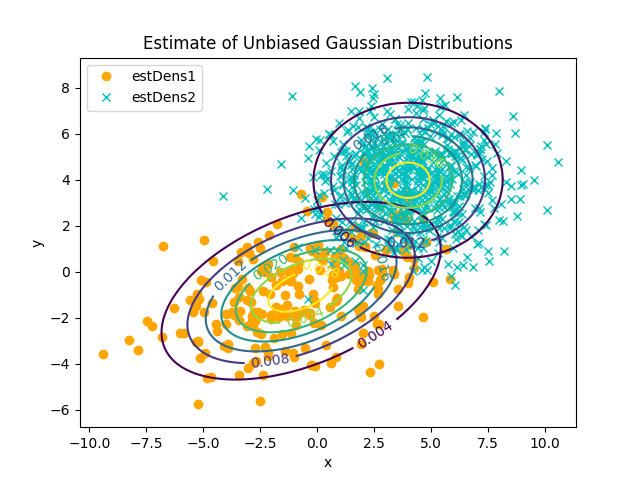
\includegraphics[scale=.7]{./Estimate.png}
	\end{subsection}
	\newpage
	\begin{subsection}*{e)}
		
		
		
		
		This plot shows the contour lines for $p(C_1\mid x)- p(C_2\mid x)$, i.e. 0 is the decision boundary, if the value is positive it is more likely, that the point is in $C_1$.
		If it is negative, $C_2$, respectively.
		
		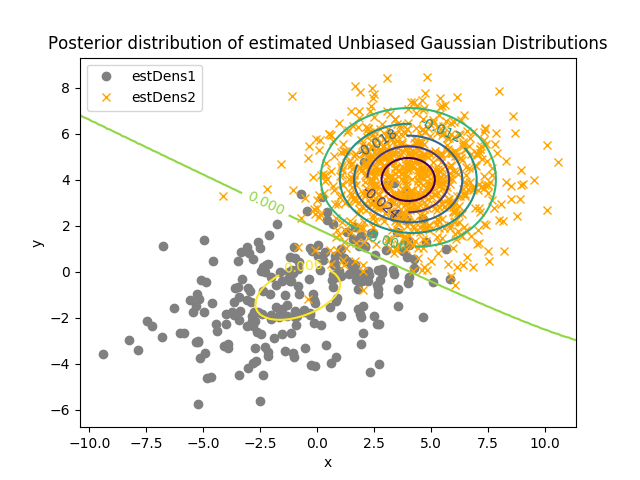
\includegraphics[scale=.7]{./Posterior.png}
	\end{subsection}
	
	\begin{subsection}*{f)}
		content...
	\end{subsection}
\end{section}

\begin{section}*{2.3 Non-parametric Density Estimation [20 Points]}
	\begin{subsection}*{a)}
		The histogram with bin size 0.02 seems overfitted and is showing a couple of gaps.
		The histogram with bin size 2.0 has too large bins and does not reflect the distribution of the training data very well. 
		As a consequence, the histogram with bin size 0.5, is the best out of these three histograms.
		However, it is possible that any bin size in between the above is able to represent the data even better.		
		Further, the distribution from which the data was samples could be highly skewed and the histogram with bin size 0.02 could be the best, even though this is unlikely. 
		
		\begin{figure}
			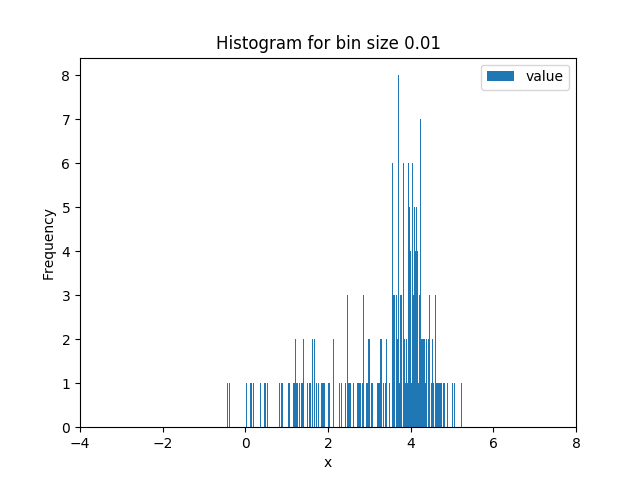
\includegraphics[scale=.4]{./hist_001}
			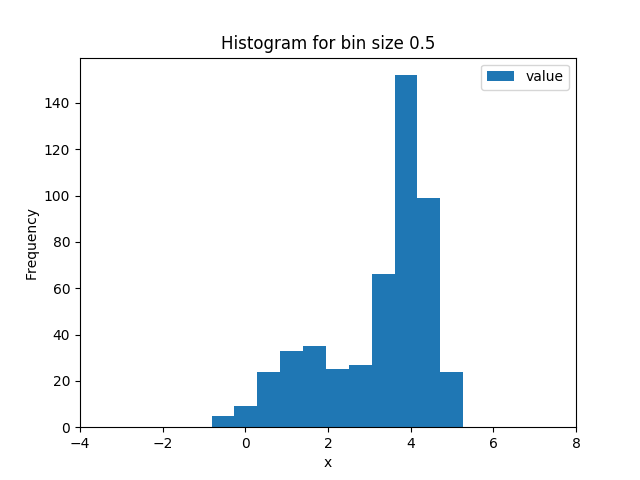
\includegraphics[scale=.4]{./hist_05}
			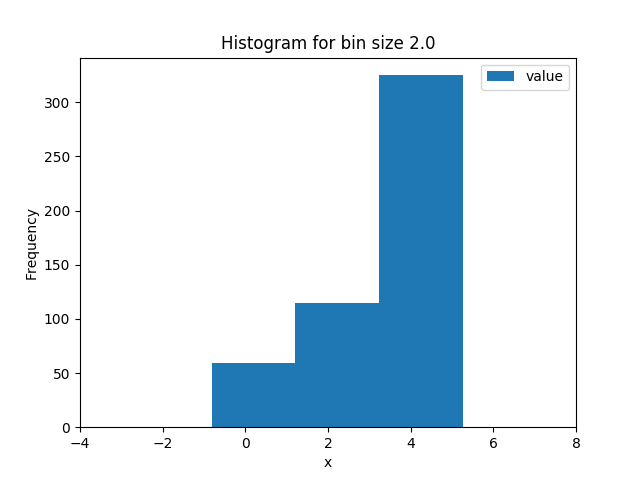
\includegraphics[scale=.4]{./hist_2}
		\end{figure}
		
		\newpage
		\begin{lstlisting}[language=python,frame=single]
import math
import pandas as pd	

x_min = -4
x_max = 8	

training_data = pd.read_csv("nonParamTrain.txt",sep="\s{2}")
training_data.columns = ["x"]

def plot_histo():

	hist_size = [0.01, 0.5, 2.]
	
	for i, s in enumerate(hist_size):
		plt.figure(i)
		train.plot.hist(by="x", 
			bins=math.ceil(
			training_data.max().value / s))
		plt.xlabel("x")
		plt.title("Histogram for bin size {}".format(s))
		plt.xlim(x_min, x_max)
	plt.show()
		\end{lstlisting}
	\end{subsection}
	\newpage
	\begin{subsection}*{b)}
		With Gaussian kernels the density estimates for $\sigma=0.03$ achieve a log-likelihood of $-674.2511$, for $\sigma=0.2$ of $-716.4553$ and for $\sigma=0.8$ of $-794.5703$.
		By just evaluating on the training data, the kernel with $\sigma=0.03$ seems to perform the best.\\
		
		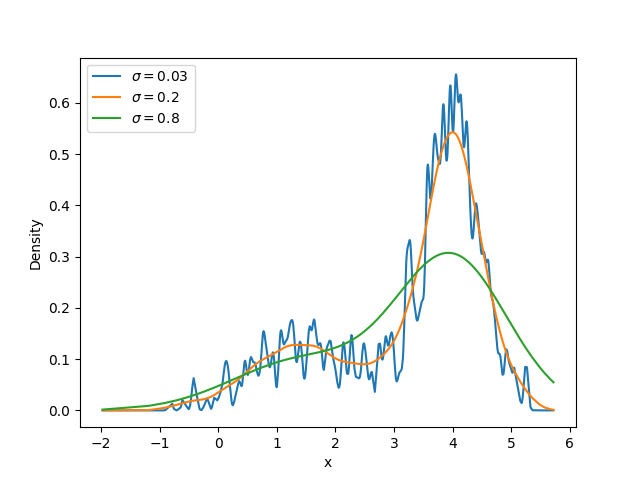
\includegraphics[scale=.7]{./KDE}
		
		\begin{lstlisting}[language=python,frame=single]
import numpy as np
import pandas as pd

x_min = -4
x_max = 8

training_data = pd.read_csv("nonParamTrain.txt",sep="\s{2}")
training_data.columns = ["x"]
		
def gaussian_kernel(x, data, sigma):

	numerator = np.sum(np.exp(-(x - data) ** 2 /
					 (2 * sigma ** 2)))
	denominator = np.sqrt(2 * math.pi) * len(data) * sigma
	return numerator / denominator
		
		
def gaussian_KDE():
	sigmas = [.03, .2, .8]
	steps = (x_max - x_min) / 500
	x = np.arange(x_min, x_max, steps)
	plt.figure()
	for sigma in sigmas:
		
		# compute kernel value for each datapoint
		y = np.empty(training_data.values.shape)
		for i, val in enumerate(training_data.values):
			y[i] = gaussian_kernel(val,
		 training_data.values, sigma)
		
		# compute log-likelihood
		print("The train log−likelihood"
		 "for $\sigma$={} is {}".format(sigma,
		   np.sum(np.log(y))))
		
		# plot for each sigma
		plt.plot(x, y, label="$\sigma={}$".format(sigma))
		plt.ylabel('Density')
		plt.xlabel('x')
		
		plt.legend()
		plt.show()
		
			content...
		\end{lstlisting}
		
	\end{subsection}
\end{section}
 
\end{document}